\documentclass[11pt]{beamer}
\usetheme{Frankfurt}
\usepackage[latin1]{inputenc}
\usepackage[T1]{fontenc}
\usepackage{appendixnumberbeamer}

\usepackage{multirow}
\usepackage{adjustbox}
\usepackage{hyperref}

\usepackage{tikz}

\usetikzlibrary{arrows, backgrounds, positioning, fit, matrix}

\usepackage{gitdags}
\usepackage{color}
\usepackage{listings}

\newcommand\Small{\fontsize{8}{8.0}\selectfont}
\newcommand*\LSTfont{\Small\ttfamily}


\definecolor{mygreen}{rgb}{0,0.6,0}
\definecolor{mygray}{gray}{0.95}

\lstset{
    language=sh,
    basicstyle=\LSTfont,
    backgroundcolor=\color{mygray},
    showspaces=false,
    showstringspaces=false,
    showtabs=false,
    frame=single,
    rulecolor=\color{black},
    tabsize=4,
    breaklines=true,
    keywordstyle=\color{blue},
    commentstyle=\color{darkgray},
    stringstyle=\color{orange}
}

\title{Introduction into Git}
%\author{}<++>

\date{\today}

\begin{document}

\maketitle

\section{Version Control Systems}

\begin{frame}[fragile]{What is Git?}

    \emph{Git is a decentralized VCS (Version Control System).}

    \begin{figure}
        \centering
        
\includegraphics[height=0.6\textheight]{img/xkcdgit.png}
        \caption{\textit{https://xkcd.com/1597/}}
    \end{figure}

\end{frame}

\begin{frame}[fragile]{Why Git?}

    \begin{figure}
        \centering
        
\includegraphics[height=0.6\textheight]{img/does_not_simply.png}
    \end{figure}

\end{frame}

\begin{frame}[fragile]{Version Control Systems}
    \emph{Local Version Control System}
    \vspace{1cm}

    \begin{minipage}{0.49\textwidth}
        \begin{itemize}
            \item store different versions of a file
            \item simple but error prone
            \item \emph{rcs} - Revsion control system
        \end{itemize}
    \end{minipage}
    \begin{minipage}{0.49\textwidth}
    \begin{figure}
        \centering
        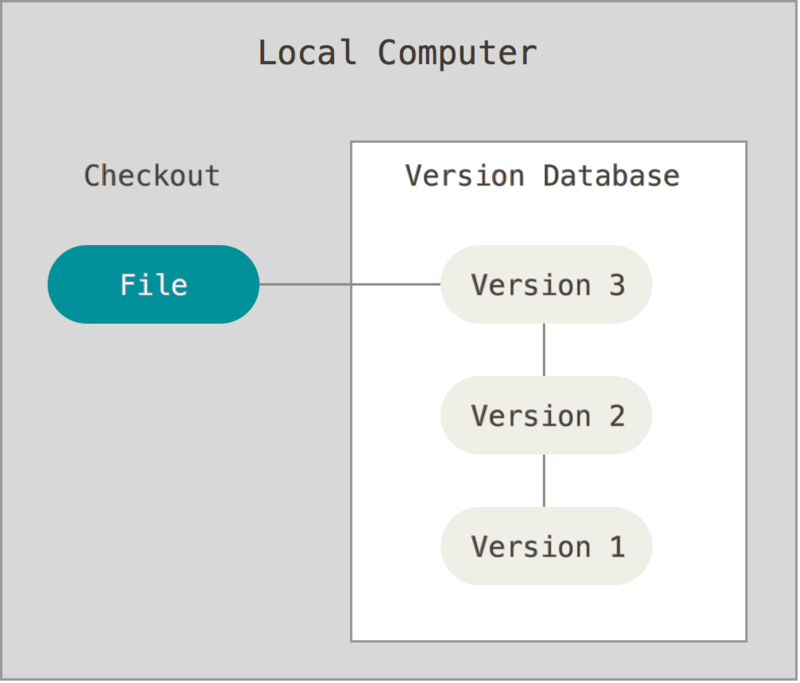
\includegraphics[width=0.9\textwidth]{img/local_vcs.png}
    \end{figure}
    \end{minipage}

\end{frame}

\begin{frame}[fragile]{Version Control System}
    \emph{Centralized Version Control Systems}
    \vspace{1cm}

    \begin{minipage}{0.49\textwidth}
        \begin{itemize}
            \item single server that conatins all the versioned files
            \item clients check out files from that central place
            \item single point of failure
            \item \emph{Subversion}, \emph{CVS}
        \end{itemize}
    \end{minipage}
    \begin{minipage}{0.49\textwidth}
        \begin{figure}
            \centering
            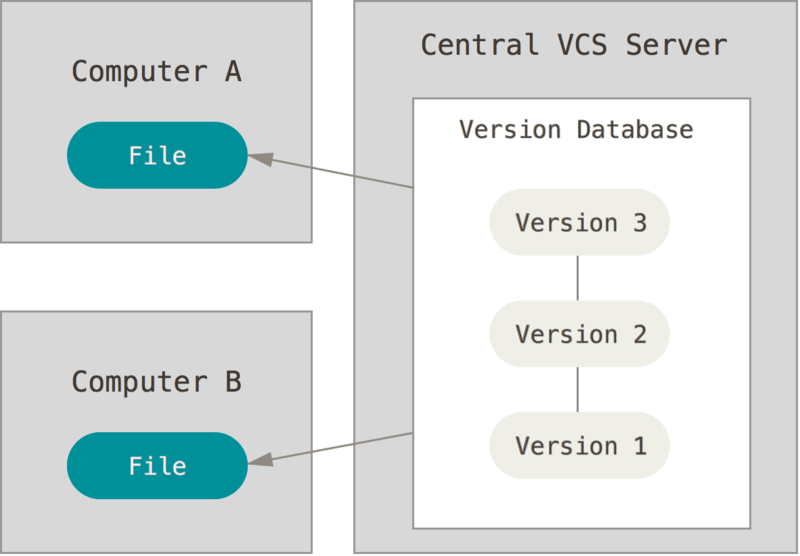
\includegraphics[width=0.9\textwidth]{img/centralized_vcs.png}
        \end{figure}
    \end{minipage}

\end{frame}

\begin{frame}[fragile]{Version Control System}
    \emph{Distributed Version Control System}
    \vspace{1cm}

    \begin{minipage}{0.49\textwidth}
        \begin{itemize}
            \item clients fully mirror the repository
            \item serveral remote repositories possible
            \item \emph{Git}, \emph{Mercurial}, \emph{Barzaar}
        \end{itemize}
    \end{minipage}
    \begin{minipage}{0.49\textwidth}
        \begin{figure}
            \centering
            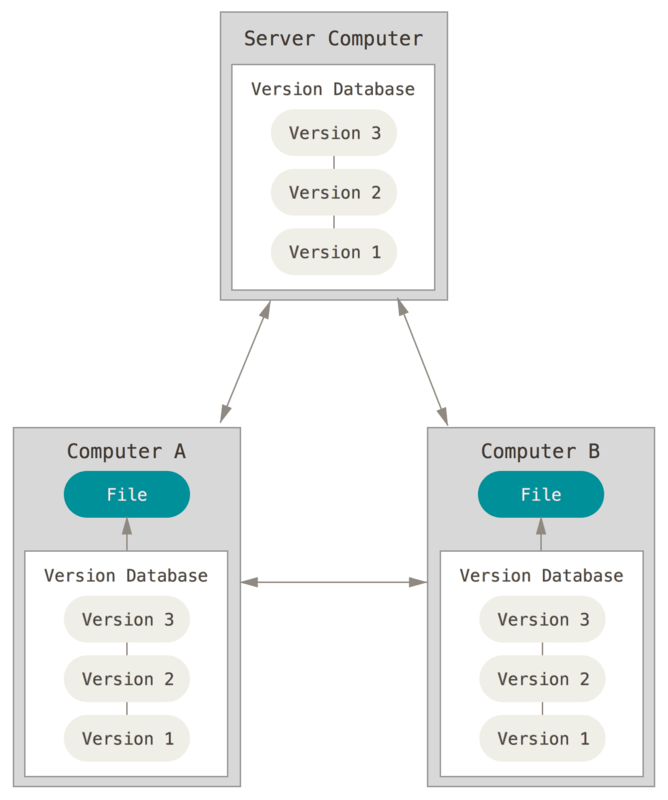
\includegraphics[width=0.9\textwidth]{img/distributed_vcs.png}
        \end{figure}
    \end{minipage}

\end{frame}

\section{Git Introduction}

\begin{frame}[fragile]{Installing git}

    \textbf{Debian:}
    \begin{lstlisting}
    apt install git
    \end{lstlisting}

    \textbf{Arch Linux:}
    \begin{lstlisting}
    pacman -S git
    \end{lstlisting}

    \textbf{Fedora:}
    \begin{lstlisting}
    dnf install git
    \end{lstlisting}

    \begin{description}
        \item{For Linux:} \url{http://git-scm.com/download/linux}
        \item{For Mac:} \url{http://git-scm.com/download/mac}
        \item{For Windows:} \url{http://git-scm.com/download/win}
    \end{description}

\end{frame}

\begin{frame}[fragile]{How it works}
    \begin{figure}
        \centering
        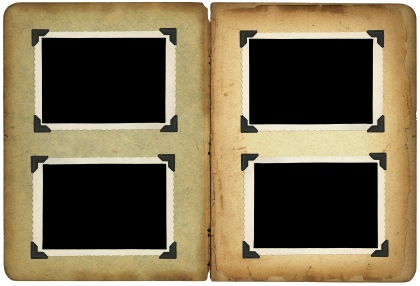
\includegraphics[width=0.8\textwidth]{img/photo_album.jpg}
        \caption{like a photo album of you work}
    \end{figure}
\end{frame}

\begin{frame}[fragile]{How it works}
    \begin{figure}
        \centering
        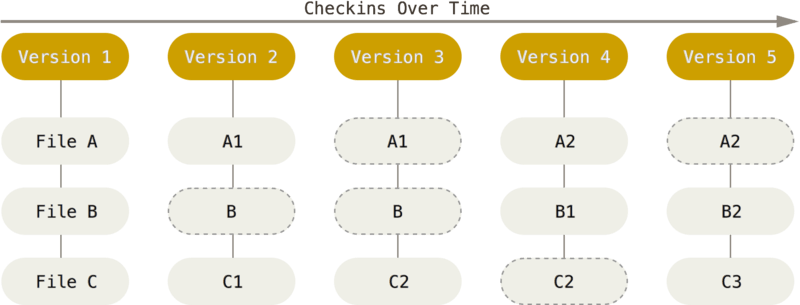
\includegraphics[width=0.8\textwidth]{img/snapshotbased.png}
        \caption{storing stream of snapshots over time}
    \end{figure}
\end{frame}

%\begin{frame}[fragile]{How it NOT works}
    %\begin{figure}
        %\centering
        %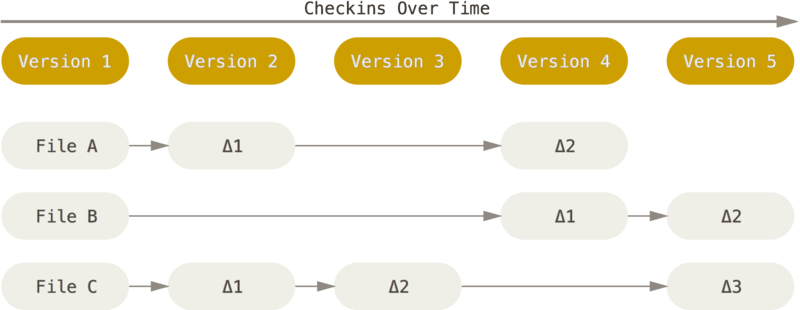
\includegraphics[width=0.8\textwidth]{img/filebased.png}
        %\caption{storing changes to a base file}
    %\end{figure}
%\end{frame}

\begin{frame}{What is a git repository?}

    \begin{figure}
        \centering
        \includegraphics[width=0.9\textwidth]{img/three_states.png}
    \end{figure}
\end{frame}

%\begin{frame}{Basic Workflow}
    %\begin{enumerate}
        %\item Modify files in your working directory.
        %\item Stage the files, adding snapshots of them to your staging area.
        %\item Commit, stores the snapshot in the staging area permanently in
            %your git directory.
        %\item Push your commits to an remote repository on a server.
    %\end{enumerate}
%\end{frame}

\defverbatim\setusername{%
    \scriptsize
    \verb+git config --global user.name "Max Mustermann"+
    \newline
}
\defverbatim\setusermail{%
    \scriptsize
    \verb+git config --global user.mail "max.mustermann@example.org"+
    \newline
}

%\begin{frame}{Configure Git}

    %\emph{Place where the git configuration can live:}
    %\vspace{1cm}

    %% TODO: take a table for that
    %\begin{itemize}
            %\item \textbf{/etc/gitconfig} system wide configuration
                %\textit{-\,-system}
            %\item \textbf{$\sim$/.gitconfig} or \textbf{$\sim$/.config/gitconfig}  user wide configuration \textit{-\,-global}
            %\item \textbf{.git/config} repository specific configuration
    %\end{itemize}

%\end{frame}

\begin{frame}[fragile]{Configure Git}
    \textbf{Show your configuration:}
    \begin{lstlisting}
        git config --list
    \end{lstlisting}
    \textbf{Show specific configuration value:}
    \begin{lstlisting}
        git config user.name
    \end{lstlisting}
    \textbf{Define an alias:}
    \begin{lstlisting}
        git config alias.st=git status
    \end{lstlisting}
    \textbf{Enable highlighting:}
    \begin{lstlisting}
        git config --global color.ui=always
    \end{lstlisting}
\end{frame}

\begin{frame}[fragile]{Setup Your Environment}
    \emph{Three essentail configuration values you should have set.}
    \vspace{1cm}

    \textbf{Your name:}
    \begin{lstlisting}
        git config --global user.name "Max Mustermann"
    \end{lstlisting}
    \textbf{Your email address:}
    \begin{lstlisting}
        git config --global user.mail "max@example.org"
    \end{lstlisting}
    \textbf{Your editor:}
    \begin{lstlisting}
        git config --global core.editor "vim"
    \end{lstlisting}
\end{frame}

\begin{frame}[fragile]{Lets Start\ldots}
    \textbf{Start from scratch:}
    \begin{lstlisting}
mkdir my_new_project
cd my_new_project
git init
    \end{lstlisting}
    \textbf{Get a local copy of a repository that already exist.}
    \begin{lstlisting}
git clone https://github.com/blastmaster/ta-git_intro.git
git clone -b <branchname> <GIT_URL>
    \end{lstlisting}
\end{frame}

%\begin{frame}[fragile]{Follow the changes}
    %\textbf{What is the status of your local repo?}
    %\begin{lstlisting}
        %git status
    %\end{lstlisting}
    %\textbf{What happens so far?}
    %\begin{lstlisting}
        %git log
    %\end{lstlisting}
    %\textbf{What has changed?}
    %\begin{lstlisting}
        %git diff [--staged]
    %\end{lstlisting}
    %\textbf{Who has changed?}
    %\begin{lstlisting}
        %git blame
    %\end{lstlisting}
%\end{frame}

%\begin{frame}[fragile]{Ignoring Files}
    %\emph{Ignore files that follow a specific pattern with a \textbf{.gitignore} file}

    %\textit{.gitignore} rules:
    %\begin{itemize}
        %\item Black lines or lines starting with \# are ignored.
        %\item Standard glob pattern work.
        %\item You can start patterns with a forward slash (/) to avoid recusivity.
        %\item You can negate a pattern by starting it with an exclamation point (!).
    %\end{itemize}

    %\vspace{1em}
    %Example:\\
    %\url{https://github.com/github/gitignore}

%\end{frame}

\section{Git local}

\begin{frame}{Recording Changes}
    \emph{Each file in your working directory can be in one of two states:
        tracked or untracked.}

    \begin{figure}
        \centering
            \includegraphics[width=\textwidth]{img/file_lifecycle.png}
    \end{figure}

\end{frame}

\begin{frame}[fragile]{Git Terminology}
    \begin{figure}[b]
        \centering
        \begin{tikzpicture}
            \tikzstyle{state} = [ draw,
                node distance = 1.4em,
                drop shadow = {opacity=0.15},
                font = \fontfamily{lmtt}\selectfont\small,
                shape = rectangle,
                %rounded corners = .5em,
                minimum width = 4cm,
                minimum height = 2em,
                text opacity = 0.75,
                semithick ]
            \tikzstyle{whatis} = [
                node distance = 1.4em,
                left,
                font = \fontfamily{lmtt}\selectfont\tiny]
            \node[state] (remote) {Remote};
            \node[state] (repository) [below=of remote] {Local Repository};
            \node[state] (index) [below=of repository] {Staging Area};
            %\node[state] (stash) [below=of index] {Stash};
            \node[state] (tree)  [below=of index] {Working Directory};

            \node[whatis, left] at (remote.west) {Repository on the internet or network.};
            \node[whatis, left] at (repository.west) {Local repository that contains complete history.};
            \node[whatis, left] at (index.west) {Snapshot of the working tree for next commit.};
            %\node[whatis, left] at (stash.west) {A place to hide modification if you need a clean workspace.};
            \node[whatis, left] at (tree.west) {The direcotries and files on your filesystem.};
        \end{tikzpicture}
    \end{figure}
\end{frame}

\begin{frame}[fragile]{Basic Workflow}
    \begin{enumerate}
        \item work in your \emph{working directory}
        \item \emph{add} changes to \emph{staging area}
        \item \emph{commit} into \emph{local repository}
        \item \emph{push} to \emph{remote}
    \end{enumerate}
\end{frame}

\begin{frame}[fragile]{Staging files}
    \begin{figure}[b]
        \centering
        \begin{tikzpicture}
            \tikzstyle{state} = [ draw,
                node distance = 1.4em,
                drop shadow = {opacity=0.15},
                font = \fontfamily{lmtt}\selectfont\small,
                shape = rectangle,
                %rounded corners = .5em,
                minimum height = 2em,
                minimum width = 4cm,
                text opacity = 0.75,
                semithick ]
            \tikzstyle{whatis} = [
                node distance = 1.4em,
                font = \fontfamily{lmtt}\selectfont\tiny]
            \node[state] (index) {Staging Area};
            \node[state] (tree)  [below=of index] {Working Directory}
                edge [->, out=0, in=0] node[whatis, right] {git add <filename>} (index)
                edge [<-, out=180, in=180] node[whatis, left] {git reset HEAD <filename>} (index);
        \end{tikzpicture}
    \end{figure}
\end{frame}

%\begin{frame}[fragile]{Using the Stash}
    %\begin{figure}[b]
        %\centering
        %\begin{tikzpicture}
            %\tikzstyle{state} = [ draw,
                %node distance = 1.4em,
                %drop shadow = {opacity=0.15},
                %font = \fontfamily{lmtt}\selectfont\small,
                %shape = rectangle,
                %%rounded corners = .5em,
                %minimum height = 2em,
                %minimum width = 4cm,
                %text opacity = 0.75,
                %semithick ]
            %\tikzstyle{whatis} = [
                %node distance = 1.4em,
                %font = \fontfamily{lmtt}\selectfont\tiny]
            %\node[state] (stash) [below=of index] {Stash};
            %\node[state] (tree)  [below=of stash] {Working Directory}
                %edge [->, out=0, in=0] node [whatis, right] {git stash} (stash)
                %edge [<-, out=180, in=180] node [whatis, left] {git stash apply} (stash);
        %\end{tikzpicture}
    %\end{figure}
%\end{frame}

\begin{frame}[fragile]{Commit Changes}
    \begin{figure}[b]
        \centering
        \begin{tikzpicture}
            \tikzstyle{state} = [ draw,
                node distance = 1.4em,
                drop shadow = {opacity=0.15},
                font = \fontfamily{lmtt}\selectfont\small,
                shape = rectangle,
                %rounded corners = .5em,
                minimum height = 2em,
                minimum width = 4cm,
                text opacity = 0.75,
                semithick ]
            \tikzstyle{whatis} = [
                node distance = 1.4em,
                font = \fontfamily{lmtt}\selectfont\tiny]
            \node[state] (repository)  {Local Repository};
            \node[state] (index) [below=of repository] {Staging Area}
                edge [->, out=0, in=0] node [whatis, right] {git commit} (repository);
            \node[state] (tree)  [below=of index] {Working Directory}
                edge [<-, out=180, in=180] node [whatis, left] {git checkout <commitid>} (repository)
                edge [->, out=0, in=0] node[whatis, right] {git add <filename>} (index);
        \end{tikzpicture}
    \end{figure}
\end{frame}

\begin{frame}[fragile]{Undoing things}

    \textbf{Unstating a Staged File:}
    \begin{lstlisting}
        git reset HEAD <file>
    \end{lstlisting}
    \textbf{Unmodifying a Modified File:}
    \begin{lstlisting}
        git checkout -- <file>
    \end{lstlisting}

\end{frame}

\section{Remotes}

\begin{frame}[fragile]{Working Remotes}
    \begin{figure}[b]
        \centering
        \begin{tikzpicture}
            \tikzstyle{state} = [ draw,
                node distance = 1.4em,
                drop shadow = {opacity=0.15},
                font = \fontfamily{lmtt}\selectfont\small,
                shape = rectangle,
                %rounded corners = .5em,
                minimum height = 2em,
                minimum width = 4cm,
                text opacity = 0.75,
            semithick ]
            \tikzstyle{whatis} = [
                node distance = 1.4em,
                font = \fontfamily{lmtt}\selectfont\tiny]
                \node[state] (remote) {Remote: origin};
                \node[state] (working) [below=of remote] {Local Repository}
                edge [<-, in=0, out=0]  node[whatis, right] {git fetch origin master} (remote)
                edge [->, in=180, out=180] node[whatis, left] {git push origin master} (remote);
        \end{tikzpicture}
    \end{figure}
\end{frame}


%\defverbatim\myadd{%
    %\scriptsize
    %\verb+git remote add github git@github.com:username/repo.git+
    %\newline
%}

%\begin{frame}[fragile]{Working with Remotes}
    %\myadd
    %\begin{figure}
        %\centering
        %\begin{tikzpicture}
            %\tikzstyle{state} = [ draw,
                %node distance = 1.4em,
                %drop shadow = {opacity=0.15},
                %font = \fontfamily{lmtt}\selectfont\small,
                %shape = rectangle,
                %%rounded corners = .5em,
                %minimum height = 2em,
                %minimum width = 4cm,
                %text opacity = 0.75,
            %semithick ]
            %\tikzstyle{whatis} = [
                %node distance = 2.4em,
                %font = \fontfamily{lmtt}\selectfont\tiny]
                %\node[state] (remote) {remote: origin};
                %\node[state] (remote2) [right=of remote] {remote: github};
                %\node[state] (working) [below=of remote, xshift=1.25cm] {local copy}
                %edge [<->, in=180, out=180] node[whatis, left, align=center] {
                    %git pull origin master \\
                %git push origin master} (remote)
                %edge [<->, in=0, out=0] node[whatis, right, align=center] {git pull github master \\
                %git push github master} (remote2);
        %\end{tikzpicture}
    %\end{figure}
%\end{frame}

\begin{frame}[fragile]{Working with Remotes}
    \textbf{Showing your remotes:}
    \begin{lstlisting}
        git remote -v
    \end{lstlisting}
    \textbf{Showing remote information:}
    \begin{lstlisting}
        git remote show <remote>
    \end{lstlisting}
    \textbf{Rename a remote:}
    \begin{lstlisting}
        git remote rename <oldname> <newname>
    \end{lstlisting}
    \textbf{Remove a remote:}
    \begin{lstlisting}
        git remote rm <remote>
    \end{lstlisting}

\end{frame}


\begin{frame}[fragile]{Commit history}
    \begin{minipage}{0.49\textwidth}
        \begin{figure}
            \begin{tikzpicture}
                \visible<-1>{
                    \gitDAG[grow right sep = 2em]
                    {
                        A
                    };
                    \gitbranch {master}
                    {below=of A}
                    {A}
                    \gitHEAD
                    {above=of A}
                    {A}
                }
                \visible<2>{
                    \gitDAG[grow right sep = 2em]
                    {
                        A -- B
                    };
                    \gitbranch {master}
                    {below=of A}
                    {A}
                    \gitHEAD
                    {above=of B}
                    {B}
                }
            \end{tikzpicture}
        \end{figure}
    \end{minipage}
    \begin{minipage}{0.49\textwidth}
        \begin{itemize}
            \visible<1->{
                \item \texttt{git add}
                \item \texttt{git commit}
            }
            \visible<2->{
                \item \texttt{git add}
                \item \texttt{git commit}
            }
        \end{itemize}
    \end{minipage}
\end{frame}

\section{Branches}

\begin{frame}[fragile]{Branching}
    \begin{minipage}{0.59\textwidth}
    \begin{figure}[b]
        \centering
        \begin{tikzpicture}
            \visible<-1>
            {
                \gitDAG[grow right sep = 2em]
                {
                    A -- B
                };
                \gitbranch {master}
                {below=of A}
                {A}
                \gitHEAD
                {above=of B}
                {B}
            }
            \visible<2->
            {
                %TODO
                \gitDAG[grow right sep = 2em]
                {
                    A -- B -- {
                        D,
                    }
                };
                \gitbranch {master}
                {below=of A}
                {A}
                \gitbranch
                {feature-X}
                {below=of D}
                {D}
                \gitHEAD
                {above=of D}
                {D}
            }
        \end{tikzpicture}
    \end{figure}
    \end{minipage}
    \begin{minipage}{0.39\textwidth}
        \begin{itemize}
                \item \texttt{git branch feature-X}
                \item \texttt{git checkout feature-X}
                \item \texttt{git add}
                \item \texttt{git commit}
        \end{itemize}
    \end{minipage}
\end{frame}

\begin{frame}[fragile]{Branching}
    \begin{minipage}{0.59\textwidth}
        \begin{figure}[b]
            \centering
            \begin{tikzpicture}
                \visible<1>
                {
                    \gitDAG[grow right sep = 2em]
                    {
                        A -- B -- {
                            C,
                            D,
                        }

                    };
                    \gitbranch {master}
                    {below=of A}
                    {A}
                    \gitbranch
                    {feature-X}
                    {below=of D}
                    {D}
                    \gitHEAD
                    {above=of C}
                    {C}
                }
                \visible<2->
                {
                    \gitDAG[grow right sep = 2em]
                    {
                        A -- B -- {
                            C,
                            D -- E,
                        }

                    };
                    \gitbranch {master}
                    {below=of A}
                    {A}
                    \gitbranch
                    {feature-X}
                    {below=of D}
                    {D}
                    \gitHEAD
                    {above=of E}
                    {E}
                }
            \end{tikzpicture}
        \end{figure}
    \end{minipage}
    \begin{minipage}{0.39\textwidth}
        \begin{itemize}
                \visible<1>
                {
                    \item \texttt{git checkout master}
                    \item \texttt{git add}
                    \item \texttt{git commit}
                }
                \visible<2->
                {
                    \item \texttt{git checkout feature-X}
                    \item \texttt{git add}
                    \item \texttt{git commit}
                }
        \end{itemize}
    \end{minipage}
\end{frame}

\begin{frame}[fragile]{Branch Syntax}
    \textbf{create new branch:}
        \begin{lstlisting}
            git branch <branchname>
        \end{lstlisting}
        \begin{lstlisting}
            git checkout -b <branchname>
        \end{lstlisting}
    \textbf{delete branch:}
        \begin{lstlisting}
            git branch -d <branchname>
        \end{lstlisting}
    \textbf{list local branches:}
        \begin{lstlisting}
            git branch
            git branch --merged
            git branch --no-merged
        \end{lstlisting}
\end{frame}

% demonstrate merging of two branches
\begin{frame}[fragile]{Merging}
        \begin{figure}
            \centering
            \begin{tikzpicture}
                \gitDAG[grow right sep = 2em]
                {
                    A -- B -- {
                        C,
                        D -- E,
                    }
                };
                \gitbranch
                {master}
                {below=of A}
                {A}
                \gitbranch
                {feature-X}
                {below=of D}
                {D}
                {feature X}
                \gitHEAD
                {above=of C}
                {C}
            \end{tikzpicture}
            \caption{Before merge\ldots}
        \end{figure}
\end{frame}

\begin{frame}[fragile]{Merging}
    \begin{figure}[b]
        \centering
        \begin{tikzpicture}
            \gitDAG[grow right sep = 2em]
            {
                A -- B --{
                C,
                    {D -- E},
                } -- E'
            };
            \gitbranch
            {master}
            {below=of A}
            {A}
            \gitbranch
            {feature-X}
            {below=of D}
            {D}
            \gitHEAD
            {above=of E'}
            {E'}
        \end{tikzpicture}
        \caption{after: \texttt{git merge feature-X}}
    \end{figure}
\end{frame}

\begin{frame}[fragile]{Rebasing}
    \begin{figure}
        \centering
        \begin{tikzpicture}
            \gitDAG[grow right sep = 2em]
            {
                A -- B -- {
                    C,
                    D -- E,
                }
            };
            \gitbranch
            {master}
            {below=of A}
            {A}
            \gitbranch
            {feature-X}
            {below=of D}
            {D}
            \gitHEAD
            {above=of C}
            {C}
        \end{tikzpicture}
        \caption{Before rebase\ldots}
    \end{figure}
\end{frame}

\begin{frame}[fragile]{Rebasing}
    \begin{figure}
        \centering
        \begin{tikzpicture}
            \gitDAG[grow right sep = 2em] {
                A -- B -- {
                    C -- D' -- E',
                    {[nodes=unreachable] D -- E},
                }
            };
            \gitbranch
            {master}
            {below=of A}
            {A}
            \gitHEAD
            {above=of E'}
            {E'}
        \end{tikzpicture}
        \caption{After \texttt{git rebase feature-X}}
    \end{figure}
\end{frame}



%\begin{frame}[fragile]{Working with the log}
    %\centering
    %\adjustbox{max height=\dimexpr\textheight-5.5cm\relax,
               %max width=\textwidth}{
    %\begin{tabular}{ll}
        %\textbf{Option} & \textbf{Description} \\ \hline
        %\textit{-(n)} & Show only the last $n$ commits\\ \hline
        %\textit{-\,-since, -\,-after} & Limit the commits to those made after the specified date.\\ \hline
        %\textit{-\,-unitl, -\,-before} & Limit the commit to those made before the specified date.\\ \hline
        %\textit{-\,-author} & Only show commits in which the author entry matches specified string.\\ \hline
        %\textit{-\,-committer} & Only show commits in which the committer entry matches the specified string.\\ \hline
        %\textit{-\,-grep} & Only show commits with a commit message containing the string.\\ \hline
        %\textit{-S}  & Only show commits adding or removing code matching the string.\\ \hline
    %\end{tabular}
    %}
%\end{frame}



\section{Advanced Usage}

\defverbatim\mytag{%
    \scriptsize
    \verb+git tag -a v0.1 A+
    \newline
}

\begin{frame}
    \frametitle{Tags}
    Tags are like bookmarks on commits.
    \begin{figure}[b]
        \centering
        \begin{tikzpicture}
            \gitDAG[grow right sep = 2em]
            {
                A -- B -- C
            };
            \gitbranch
            {master}
            {above=of C}
            {C}
            \gitHEAD
            {above=of master}
            {master}
        \end{tikzpicture}
    \end{figure}
\end{frame}

\begin{frame}[fragile]{Tags}
    \mytag
    \begin{figure}[b]
        \centering
        \begin{tikzpicture}
            \gitDAG[grow right sep = 2em]
            {
                A -- B -- C
            };
            \gitbranch {master}
            {above=of C}
            {C}
            \gittag
            [v0p1]
            {v0.1}
            {above=of A}
            {A}
            \gitHEAD
            {above=of master}
            {master}
        \end{tikzpicture}
    \end{figure}
\end{frame}

\begin{frame}[fragile]{Tags Syntax}
    \textbf{Create tag:}
    \begin{lstlisting}
    git tag -a <commitid>
    \end{lstlisting}
    \textbf{Delete tag:}
    \begin{lstlisting}
    git tag -d <tagname>
    \end{lstlisting}
    \textbf{Filter tag:}
    \begin{lstlisting}
    git tag -l <pattern>
    \end{lstlisting}
    \textbf{Sign tag:}
    \begin{lstlisting}
    git tag -s <tagname>
    \end{lstlisting}
    \textbf{Showing a tag:}
    \begin{lstlisting}
    git show v1.4
    \end{lstlisting}
\end{frame}

\begin{frame}[fragile]{Sharing Tags}
    \textbf{You need to explicitly transfer tags to remote.}
    \begin{lstlisting}
        git push origin <tagname>
    \end{lstlisting}
    or:
    \begin{lstlisting}
        git push origin --tags
    \end{lstlisting}
    \textbf{Checking out Tags:}
    \begin{lstlisting}
        git checkout -b <branchname> <tagname>
    \end{lstlisting}
\end{frame}


% Submodule

\begin{frame}[fragile]{Submodules}
    \emph{Submodules allow you to include or embed one or more repositories as a
        sub-folder inside another repository.}
    \vspace{1cm}


    \textbf{Adding a new submodule:}
    \begin{lstlisting}
    git submodule add <GIT_URL> <PATH>
    \end{lstlisting}
    \textbf{Update a submodule:}
    \begin{lstlisting}
    git submodule update --remote
    \end{lstlisting}

    The \textbf{.gitmodules} file stores the mapping between the projects url
    and the local subdirectory you've pulled it into.

\end{frame}

\begin{frame}[fragile]{Submodules}
    \emph{Cloning a Repository with Submodules.}
    \vspace{1cm}

    \begin{lstlisting}
    git clone <GIT_URL>
    git submodule init
    git submodule update --recursive
    \end{lstlisting}
    or shorter:
    \begin{lstlisting}
    git clone <GIT_URL>
    git submodule update --init --recursive
    \end{lstlisting}
    or even shorter:
    \begin{lstlisting}
    git clone --recursive <GIT_URL>
    \end{lstlisting}

\end{frame}

\begin{frame}[fragile]{Submodules}
    \emph{To remove a submodule you need to:}
    \vspace{1cm}

    \begin{enumerate}
        \item Delete the relevant line from the \textbf{.gitmodules} file.
        \item Delete the relevant section from \textbf{.git/config}.
        \item Run \textit{git rm -\,-cached path\_to\_submodule} (no trailing slash).
        \item Commit the superproject.
        \item Delete the now untracked submodule files.
    \end{enumerate}
\end{frame}

\section{Pitfalls}

\begin{frame}[fragile]{Oh shit, I did something terribly wrong, please tell me git has a magic time machine!?!}
    \begin{figure}
    \begin{lstlisting}
        git reflog
        # you will see a list of every thing you've done in git, across all branches!
        # each one has an index HEAD@{index}
        # find the one before you broke everything
        git reset HEAD@{index}
        # magic time machine
    \end{lstlisting}
    \end{figure}
\end{frame}

\begin{frame}[fragile]{Oh shit, I committed and immediately realized I need to make one small change!}
    \begin{figure}
    \begin{lstlisting}
        # make your change
        git add . # or add individual files
        git commit --amend
        # follow prompts to change or keep the commit message
        # now your last commit contains that change!
    \end{lstlisting}
    \end{figure}
\end{frame}

\begin{frame}[fragile]{Oh shit, I need to change the message on my last commit!}
    \begin{figure}
    \begin{lstlisting}
        git commit --amend
        # follow prompts to change the commit message
    \end{lstlisting}
    \end{figure}
\end{frame}

\begin{frame}[fragile]{Oh shit, I accidentally committed something to master that should have been on a brand new branch!}
    \begin{figure}
    \begin{lstlisting}
        # create a new branch from the current state of master
        git branch some-new-branch-name
        # remove the commit from the master branch
        git reset HEAD~ --hard
        git checkout some-new-branch-name
        # your commit lives in this branch now :)
    \end{lstlisting}
    \end{figure}
\end{frame}

\begin{frame}[fragile]{Oh shit, I accidentally committed to the wrong branch!}
    \begin{figure}
    \begin{lstlisting}
        # undo the last commit, but leave the changes available
        git reset HEAD~ --soft
        git stash
        # move to the correct branch
        git checkout name-of-the-correct-branch
        git stash pop
        git add . # or add individual files
        git commit -m "your message here"
        # now your changes are on the correct branch
        \end{lstlisting}
\end{figure}
\end{frame}

\begin{frame}[fragile]{Fuck this noise, I give up.}

    \begin{figure}
        \begin{lstlisting}
        cd ..
        rm -rf git-repo-dir
        git clone https://some.github.url/git-repo-dir.git
        cd git-repo-dir
        \end{lstlisting}
    \end{figure}
\end{frame}

\begin{frame}{End}

    \begin{figure}
    \centering
    
\includegraphics[width=\textwidth]{img/git-logo.png}
    \end{figure}

\end{frame}


\end{document}
